\documentclass[a4paper]{article}

\usepackage[T2A]{fontenc}
\usepackage[utf8]{inputenc}
\usepackage[russian]{babel}
\usepackage{graphicx}
\usepackage{float}
\usepackage{mathtools}
\usepackage{wrapfig}
\usepackage{amsfonts, amssymb, amsmath, latexsym}
\usepackage{nicefrac}
\usepackage{hhline}
\usepackage{multirow}
\usepackage[colorlinks=true,linkcolor=black,citecolor=blue]{hyperref}       % hyperlinks
\usepackage{nicefrac}       % compact symbols for 1/2, etc.
\usepackage{nameref}
\usepackage{booktabs}       % professional-quality tables
\usepackage{algorithm}
\usepackage{algpseudocode}
\usepackage{xcolor, colortbl}
\usepackage{etoolbox}

% \graphicspath{ {./} }

\usepackage[verbose=true,letterpaper]{geometry}

\newgeometry{
    textheight=25cm,
    textwidth=18cm,
    top=2.5cm,
    headheight=12pt,
    headsep=10pt,
    footskip=1cm,
    marginparwidth=15pt
}

%\usepackage{showframe} 

\usepackage{epigraph}
\usepackage{amsmath,amsfonts,amssymb,amsthm,mathtools, mathrsfs}
\usepackage{amsthm}

\title{Работа 5.5.5 \\ Компьютерная сцинтилляционная $\gamma$-спектрометрия}
\author{Шарапов Денис, Колесников Иван, Б05-004}
\date{}

\usepackage{fancyhdr}
\pagestyle{fancy}
\fancyhf{}
\rhead{Работа 5.5.5}
\lhead{}
\cfoot{\thepage}
\usepackage{subcaption}
\usepackage[font={small}]{caption}

\begin{document}

    \maketitle
    \tableofcontents
    \newpage
    
\section{Аннотация}

\noindent\textbf{Цель работы:} исследовать спектры излучения различных источников, характеризовать различные пики в спектрах радиоактивных веществ. \smallskip
 
\noindent \textbf{В работе используются:} сцинтиллятор, фотоэлектронные умножители (ФЭУ), предусилитель импульсов, высоковольтный блок питания для ФЭУ, блок преобразования аналоговых импульсов с ФЭУ в цифровой код, компьютер.

\section{Теоретические сведения}

\noindent\textbf{Фотоэффект} --- процесс взаимодействия гамма-кванта с электроном, связанным с атомом, при котором электрону передается вся энергия гаммакванта. При этом электрону сообщается кинетическая энергия $$T_e = E_{\gamma} - I_i,$$ где $E_{\gamma}$ --- энергия гамма-кванта, $I_i$ --- потенциал ионизации $i$-той оболочки атома. Фотоэффект особенно существенен для тяжелых веществ, где он идет с заметной вероятностью даже при высоких энергиях гамма-квантов. В легких веществах фотоэффект становится заметен лишь при относительно небольших энергиях гамма-квантов. Наряду с фотоэффектом, при котором вся энергия гамма-кванта передается атомному электрону, взаимодействие гаммаизлучения со средой может приводить к его рассеянию, т.е. отклонению от первоначального направления распространения на некоторый угол. \medskip

\noindent\textbf{Эффект Комптона} --- упругое рассеяние фотона на свободном электроне, сопровождающееся изменением длины волны фотона (реально этот процесс происходит на слабо связанных с атомом внешних электронах). Максимальная энергия образующихся комптоновских электронов соответствует рассеянию гамма-квантов на $180^\circ$ и равна $$E_{\text{max}} = \frac{\hbar\omega }{1 + \frac{mc^2}{2\hbar\omega}}.$$

\noindent\textbf{Процесс образования электрон-позитронных пар.} При достаточно высокой энергии гамма-кванта наряду с фотоэффектом и эффектом Комптона может происходить третий вид взаимодействия гамма-квантов с веществом --- образование электрон-позитронных пар. Процесс образования пар не может происходить в пустоте, так как в этом случае не выполняются законы сохранения энергии и импульса. В присутствии ядра или электрона процесс образования пары гамма-квантов возможен, так как можно распределить энергию и импульс гамма-кванта между тремя частицами без противоречия с законами сохранения. При этом если процесс образования пары идет в кулоновском поле ядра или протона, то энергия образующегося ядра отдачи оказывается весьма малой, так что пороговая энергия гамма-кванта $E_0$, необходимая для образования пары, практически совпадает с удвоенной энергией покоя электрона $$E_0 \approx 2mc^2=1.022 \;\; \text{МэВ}.$$ Появившийся в результате процесса образования пар электрон свою энергию на ионизацию среды. Таким образом, вся энергия электрона остается в детекторе. Позитрон будет двигаться до тех пор, пока практически не остановится, а затем аннигилирует с электроном среды, в результате чего появятся два гамма-кванта. Т.е., кинетическая энергия позитрона также останется в детекторе. Далее возможны три варианта развития событий:
\begin{enumerate}
\item оба родившихся гамма-кванта не вылетают из детектора, и тогда вся энергия первичного гамма-кванта останется в детекторе, а в спектре появится пик с $E=E_{\gamma}$;
\item один из родившихся гамма-квантов покидает детектор, и в спектре появляется пик, соответствующий энергии $E=E_{\gamma}-E_0,$ где $E_0=mc^2=511$ кэВ;
\item оба родившихся гамма-кванта покидают детектор, и в спектре появляется пик, соотвествующий энергии $E=E_{\gamma}-2E_0$, где $2E_0=2mc^2=1022$ кэВ.
\end{enumerate}
Таким образом, любой спектр, получаемый с помощью гамма-спектрометра, описывается несколькими компонентами, каждая из которых связана с определенным физическим процессом. Как описано выше, основными физическими процессами взаимодействия гамма-квантов с веществом является фотоэффект, эффект Комптона и образование электрон-позитронных пар, и каждый из них вносит свой вклад в образование спектра. Помимо этих процессов, добавляется \textit{экспонента}, связанная с наличием фона, \textit{пик характеристического излучения}, возникающий при взаимодействии гамма-квантов с окружающим веществом, а также \textit{пик обратного рассеяния}, образующийся при энергии квантов $E_{\gamma}\gg mc^2/2$ в результате рассеяния гамма-квантов на большие углы на материалах  конструктивных элементов детектора и защиты. Положение пика обратного рассеяния определяется по формуле 
\begin{equation}
    E_{\text{обр}}=\frac{E}{1+2E/mc^2},
\end{equation}
где $E$ -- энергия фотопика.

\subsection{Энергетическое разрешение спектрометра} Даже при поглощении частиц с одинаковой энергией амплитуда импульса на выходе фотоприёмника сцинтилляционного детектора меняется от события к событию. Это связано:
\begin{enumerate}
\item со статистическим характером процессов сбора фотонов на фотоприёмнике и последующего усиления,
\item с различной вероятностью доставки фотона к фотоприемнику из разных точек сцинтиллятора,
\item с разбросом высвечиваемого числа фотонов
\end{enumerate}

\noindent В результате в набранном спектре линия (которая для идеального детектора представляла бы дельта-функцию) оказывается размытой, её часто описывают гауссианом. Энергетическим разрешением спектрометра называется величина
\begin{equation}
R_i=\frac{\Delta E_i}{E_i},
\end{equation}
где $\Delta E_i$ -- ширина пика полного поглощения, измеренная на половине высоты, $E_i$ -- энергия регистрируемого $\gamma$-излучения. Значение $E_i$ пропорционально среднему числу фотонов $\overline{n_i}$ на выходе ФЭУ, т.е.:
\begin{equation}
E_i=\alpha\overline{n_i}.
\label{eq:4}
\end{equation}

\noindent Полуширина пика полного поглощения $\Delta E_i$ пропорциональна среднеквадратичной флуктуации $\overline{\Delta n_i}$. Т.к. $n_i$ является дискретной случайной величиной, которая распределена по закону Пуассона, то $\overline{\Delta n_i}=\sqrt{\overline{n_i}}$ и поэтому
\begin{equation}
\Delta E_i=\alpha\overline{\Delta n_i}=\alpha\sqrt{\overline{n_i}}.
\label{eq:5}
\end{equation}

\noindent Из (\ref{eq:4}), (\ref{eq:5}) получаем, что
\begin{equation}
R_i=\frac{\Delta E_i}{E_i}=\frac{\text{const}}{\sqrt{E_i}}.
\label{eq:6}
\end{equation}

\noindent Поскольку энергетическое разрешение зависит от энергии, его следует указывать для конкретной энергии. Чаще всего разрешение указывают для энергии гамма-линии $^{137}\text{Cs}$ ($661,7$ кэВ).

\section{Экспериментальная установка}

Принципиальная блок-схема гамма-спектрометра, изучаемого в данной работе, показана на рис. 1.

\begin{figure}[!ht]
    \begin{center}
        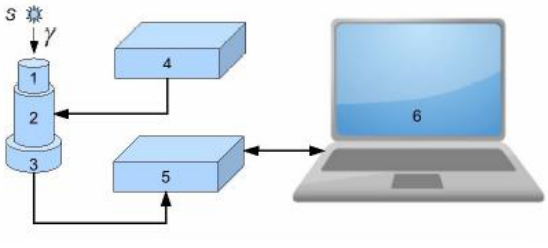
\includegraphics[width = 0.40\textwidth]{image/pic1.png}
        \caption{Принципиальная блок-схема спектрометра: 1 -- сцинтиллятор, 2 -- ФЭУ, 3 -- предусилитель импульсов, 4 -- высоковольтный блок питания для ФЭУ, 5 -- блок преобразования аналоговых импульсов с ФЭУ в цифровой код (АЦП), 6 -- компьютер для сбора данных, их обработки и хранения}
    \end{center}
\end{figure}

\section{Результаты измерений и обработка данных}

\subsection {Калибровка}

\noindent Используя известные значения (табл. 1) пиков в спектрах натрия и цезия, построим калибровочный график соответствия номера канала определённому значению энергии (рис. 2). Получаем уравнение для перехода от номера канала к значению энергии:
\begin{center}
    $E = 0.73N_i - 48,41 \;\; [\text{кэВ}].$
\end{center}

\begin{table}[!ht]
    \centering
    \caption{Известные значения пиков в спектрах натрия и цезия}
    \begin{tabular}{|c|c|c|}
    \hline
    Образец & $E$, кэВ & $N$    \\ \hline
    $^{22}$Na      & $511,0$    & $766$  \\ \hline
    $^{22}$Na      & $661,7$  & $971$  \\ \hline
    $^{137}$Cs      & $1275,0$   & $1811$ \\ \hline
    \end{tabular}
    \end{table}

\begin{figure}[!ht]
    \begin{center}
        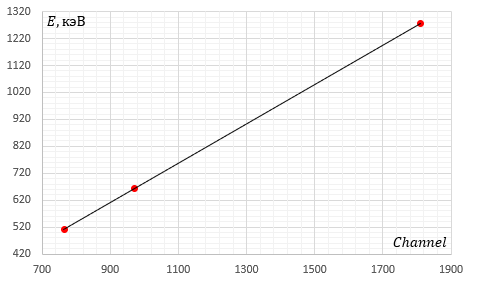
\includegraphics[width = 0.5\textwidth]{image/gr1.png}
        \caption{Калибровочный график для перехода от номера канала к значению энергии}
    \end{center}
\end{figure}


\subsection {Определение параметров образцов}

\noindent Используя калибровочный график, определим для всех остальных источников значения энергии пиков полного поглощения $E_i$, их ширины на половине высоты $\triangle E_i$ и энергетическое разрешение $R_i$. Результаты занесём в таблицу 2. В последний столбец $E$ запишем справочные значения для соответствующих энергий пиков полного поглощения.

\begin{table}[h]
    \centering
    \caption{Пики полного поглощения различных образцов}
    \label{tab:my_label}
    \begin{tabular}{|c|c|c|c|c|c|c|}
\hline
  Элемент & $N_i$ & $\Delta N_i$ & $E_i$, МэВ & $\Delta E_i$, МэВ & $R_i$ & $E$, МэВ \\
 \hline
 $^{22}$Na & 1811 & 83 & 1.274 & 0.030 & 0.023 & 1.274  \\
\hline
 $^{60}$Co & 1670 & 37 & 1.171 & 0.027 & 0.023  & 1.173 \\
\hline
 $^{60}$Co & 1892 & 45 & 1.333 & 0.033 & 0.024 & 1.332 \\
\hline
$^{137}$Cs & 967 & 62 & 0.662 & 0.022 & 0.032 & 0.662  \\
\hline
$^{241}$Am & 149 & 13 & 0.060 & 0.004 & 0.067 & 0.595 \\
\hline
$^{152}$Eu & 235 & 17 & 0.123 & 0.006 & 0.045 & 0.122 \\
\hline
$^{152}$Eu & 399 & 31 & 0.243 & 0.010 & 0.040 & 0.245 \\
\hline
$^{152}$Eu & 534 & 41 & 0.341 & 0.015 & 0.041 & 0.344 \\
\hline
 \end{tabular}
\end{table} 

\subsection{Исследование зависимости энергетического разрешения от энергии регистрируемого излучения}

\noindent Проверим зависимость (5). Для этого построим график зависимости $R^2 = f(1/E)$ (рис. 3). Наблюдается линейная зависимость. Из-за неточностей в определении полуширины пиков точки не лежат на одной прямой.

\begin{figure}[!ht]
    \begin{center}
        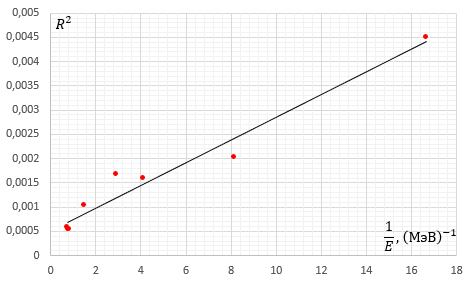
\includegraphics[width = 0.55\textwidth]{image/gr2.png}
        \caption{Зависимость энергетического разрешения от энергии регистрируемого излучения}
    \end{center}
\end{figure}

\newpage

\subsection{Энергии края комптоновского рассеяния}

\noindent Определим энергии края комптоновского поглощения для образцов $^{22}$Na, $^{137}$Cs, $^{60}$Co и сравним их с соответствующими справочными значениями. Результаты представлены в таблице 3.

\begin{table}[!ht]
    \centering
    \caption{Результаты определения энергии края комптоновского поглощения}
    \begin{tabular}{|c|c|c|}
    \hline
    Образец & $E_{\text{exp}}$, МэВ & $E_{\text{thr}}$, МэВ \\ \hline
    $^{60}$Co      & $0,922$               & $0,963$               \\ \hline
    $^{137}$Cs      & $0,448$               & $0,477$               \\ \hline
    $^{22}$Na      & $0,999$               & $1,062$               \\ \hline
    \end{tabular}
    \end{table}

\noindent В спектрах, где наблюдаются пики обратного рассеяния, определим энергии этих пиков и сравним измеренные значения с определёнными по формуле (1). Результаты представлены в таблице 4. 

\begin{table}[!ht]
    \centering
    \caption{Энергии пиков обратного рассеяния}
    \begin{tabular}{|c|c|c|}
    \hline
    Образец & $E_{\text{exp}}$, МэВ & $E_{\text{thr}}$, МэВ \\ \hline
    $^{60}$Co      & $0,228$               & $0,209$               \\ \hline
    $^{60}$Co      & $0,228$               & $0,214$               \\ \hline
    $^{137}$Cs      & $0,198$               & $0,184$               \\ \hline
    \end{tabular}
\end{table}

\noindent Эти значения практически совпадают. Пики обратного рассеяния в спектре кобальта, отвечающие разным пикам полного поглощения, на графике неразрешимы (виден один широкий пик).

\begin{figure}[!ht]
    \begin{center}
        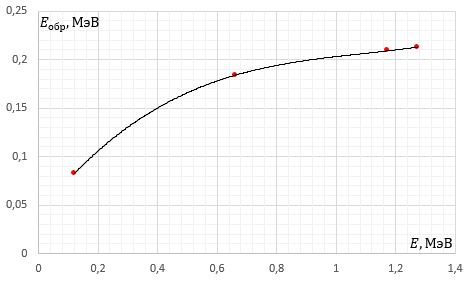
\includegraphics[width = 0.55\textwidth]{image/pic4.png}
        \caption{Пики обратного рассеяния}
    \end{center}
\end{figure}

\section{Вывод}

В ходе работы после калибровки прибора были сняты спектры образцов $^{22}$Na,  $^{60}$Cо,  $^{137}$Cs, $^{241}$Am, $^{152}$Eu. В спектрах были исследованы пики, соответствующие следующим взаимодействиям гамма-квантов с веществом:
\begin{itemize}
    \item фотоэффект (пики полного поглощения)
    \item эффект Комптона (характерное распределение энергий в спектре, оканчивающееся комптоновским краем)
    \item обратное рассеяние (пики обратного рассеяния)
    \item аннигиляция позитронов (пик 511 кэВ в спектре натрия, по которому проводилась калибровка)
\end{itemize}


\section{Приложение: спектрограммы}

\begin{figure}[ht]
\begin{center}
\begin{minipage}[h]{0.48\linewidth}
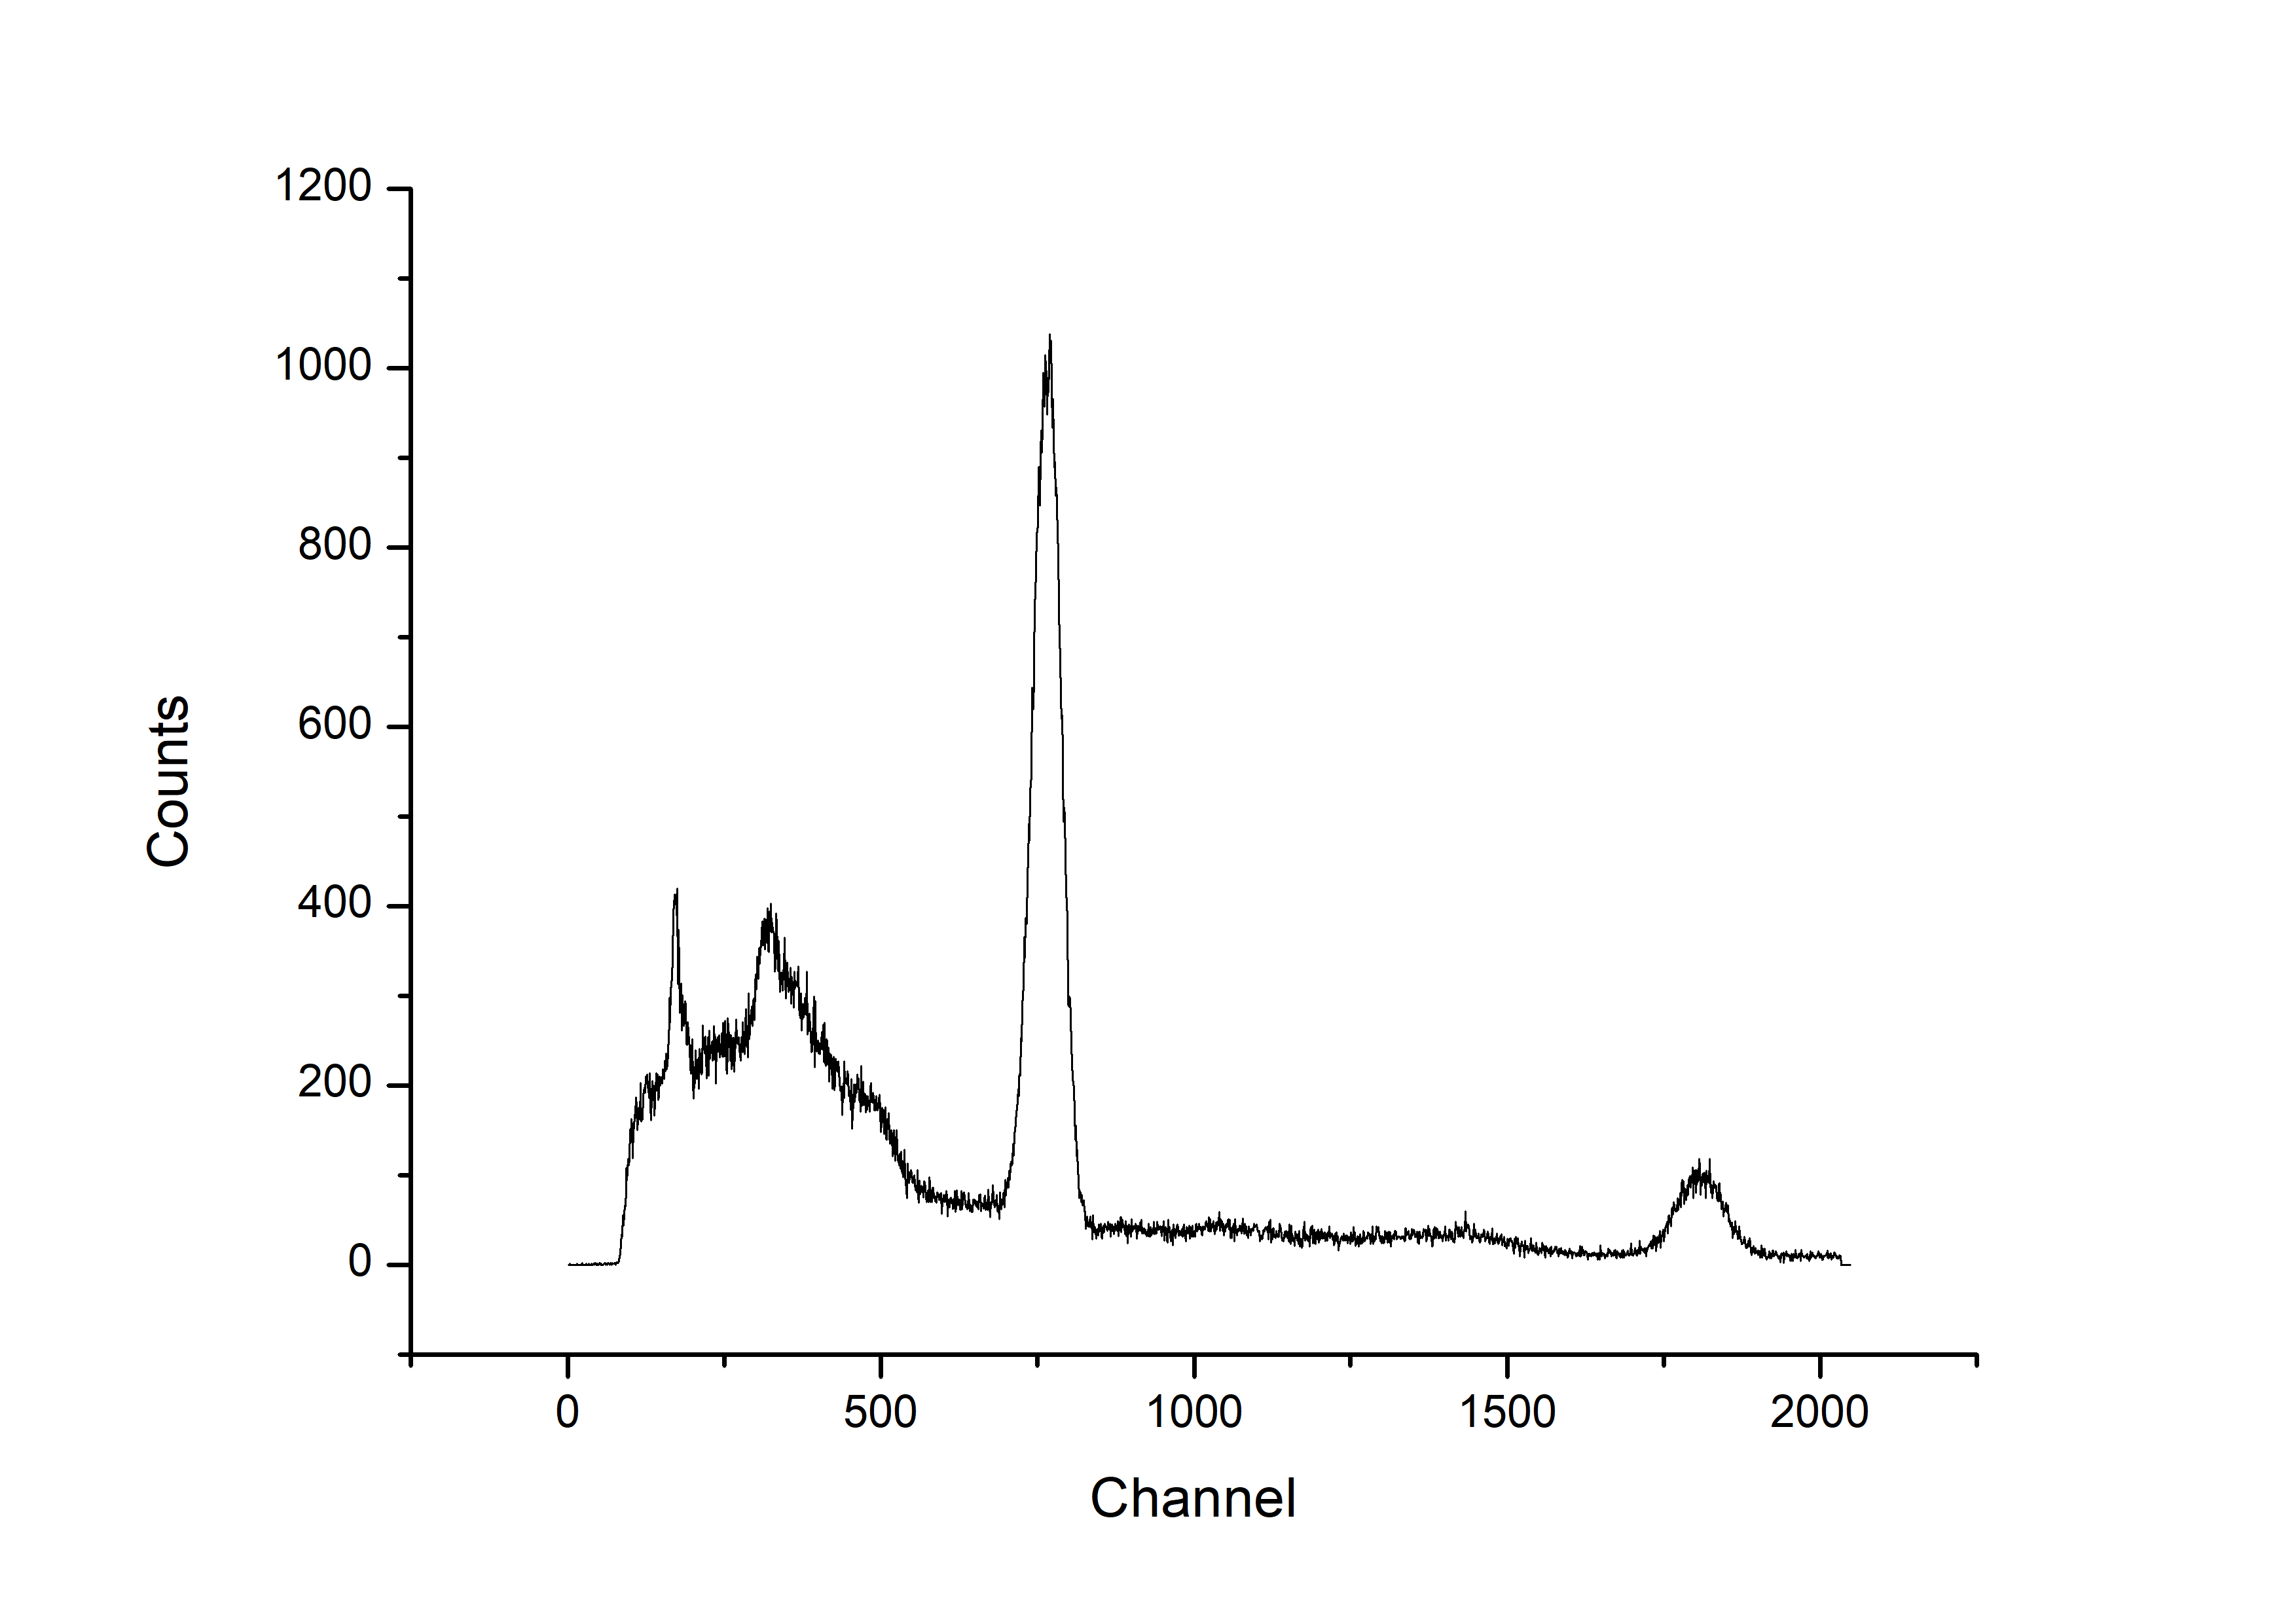
\includegraphics[width=1\linewidth]{image/Na.png}
\caption{Спектр $^{22}$Na} %% подпись к рисунку\label{ris:experimoriginal} %% метка рисунка для ссылки на него
\end{minipage}
\hfill 
\begin{minipage}[ht]{0.48\linewidth}
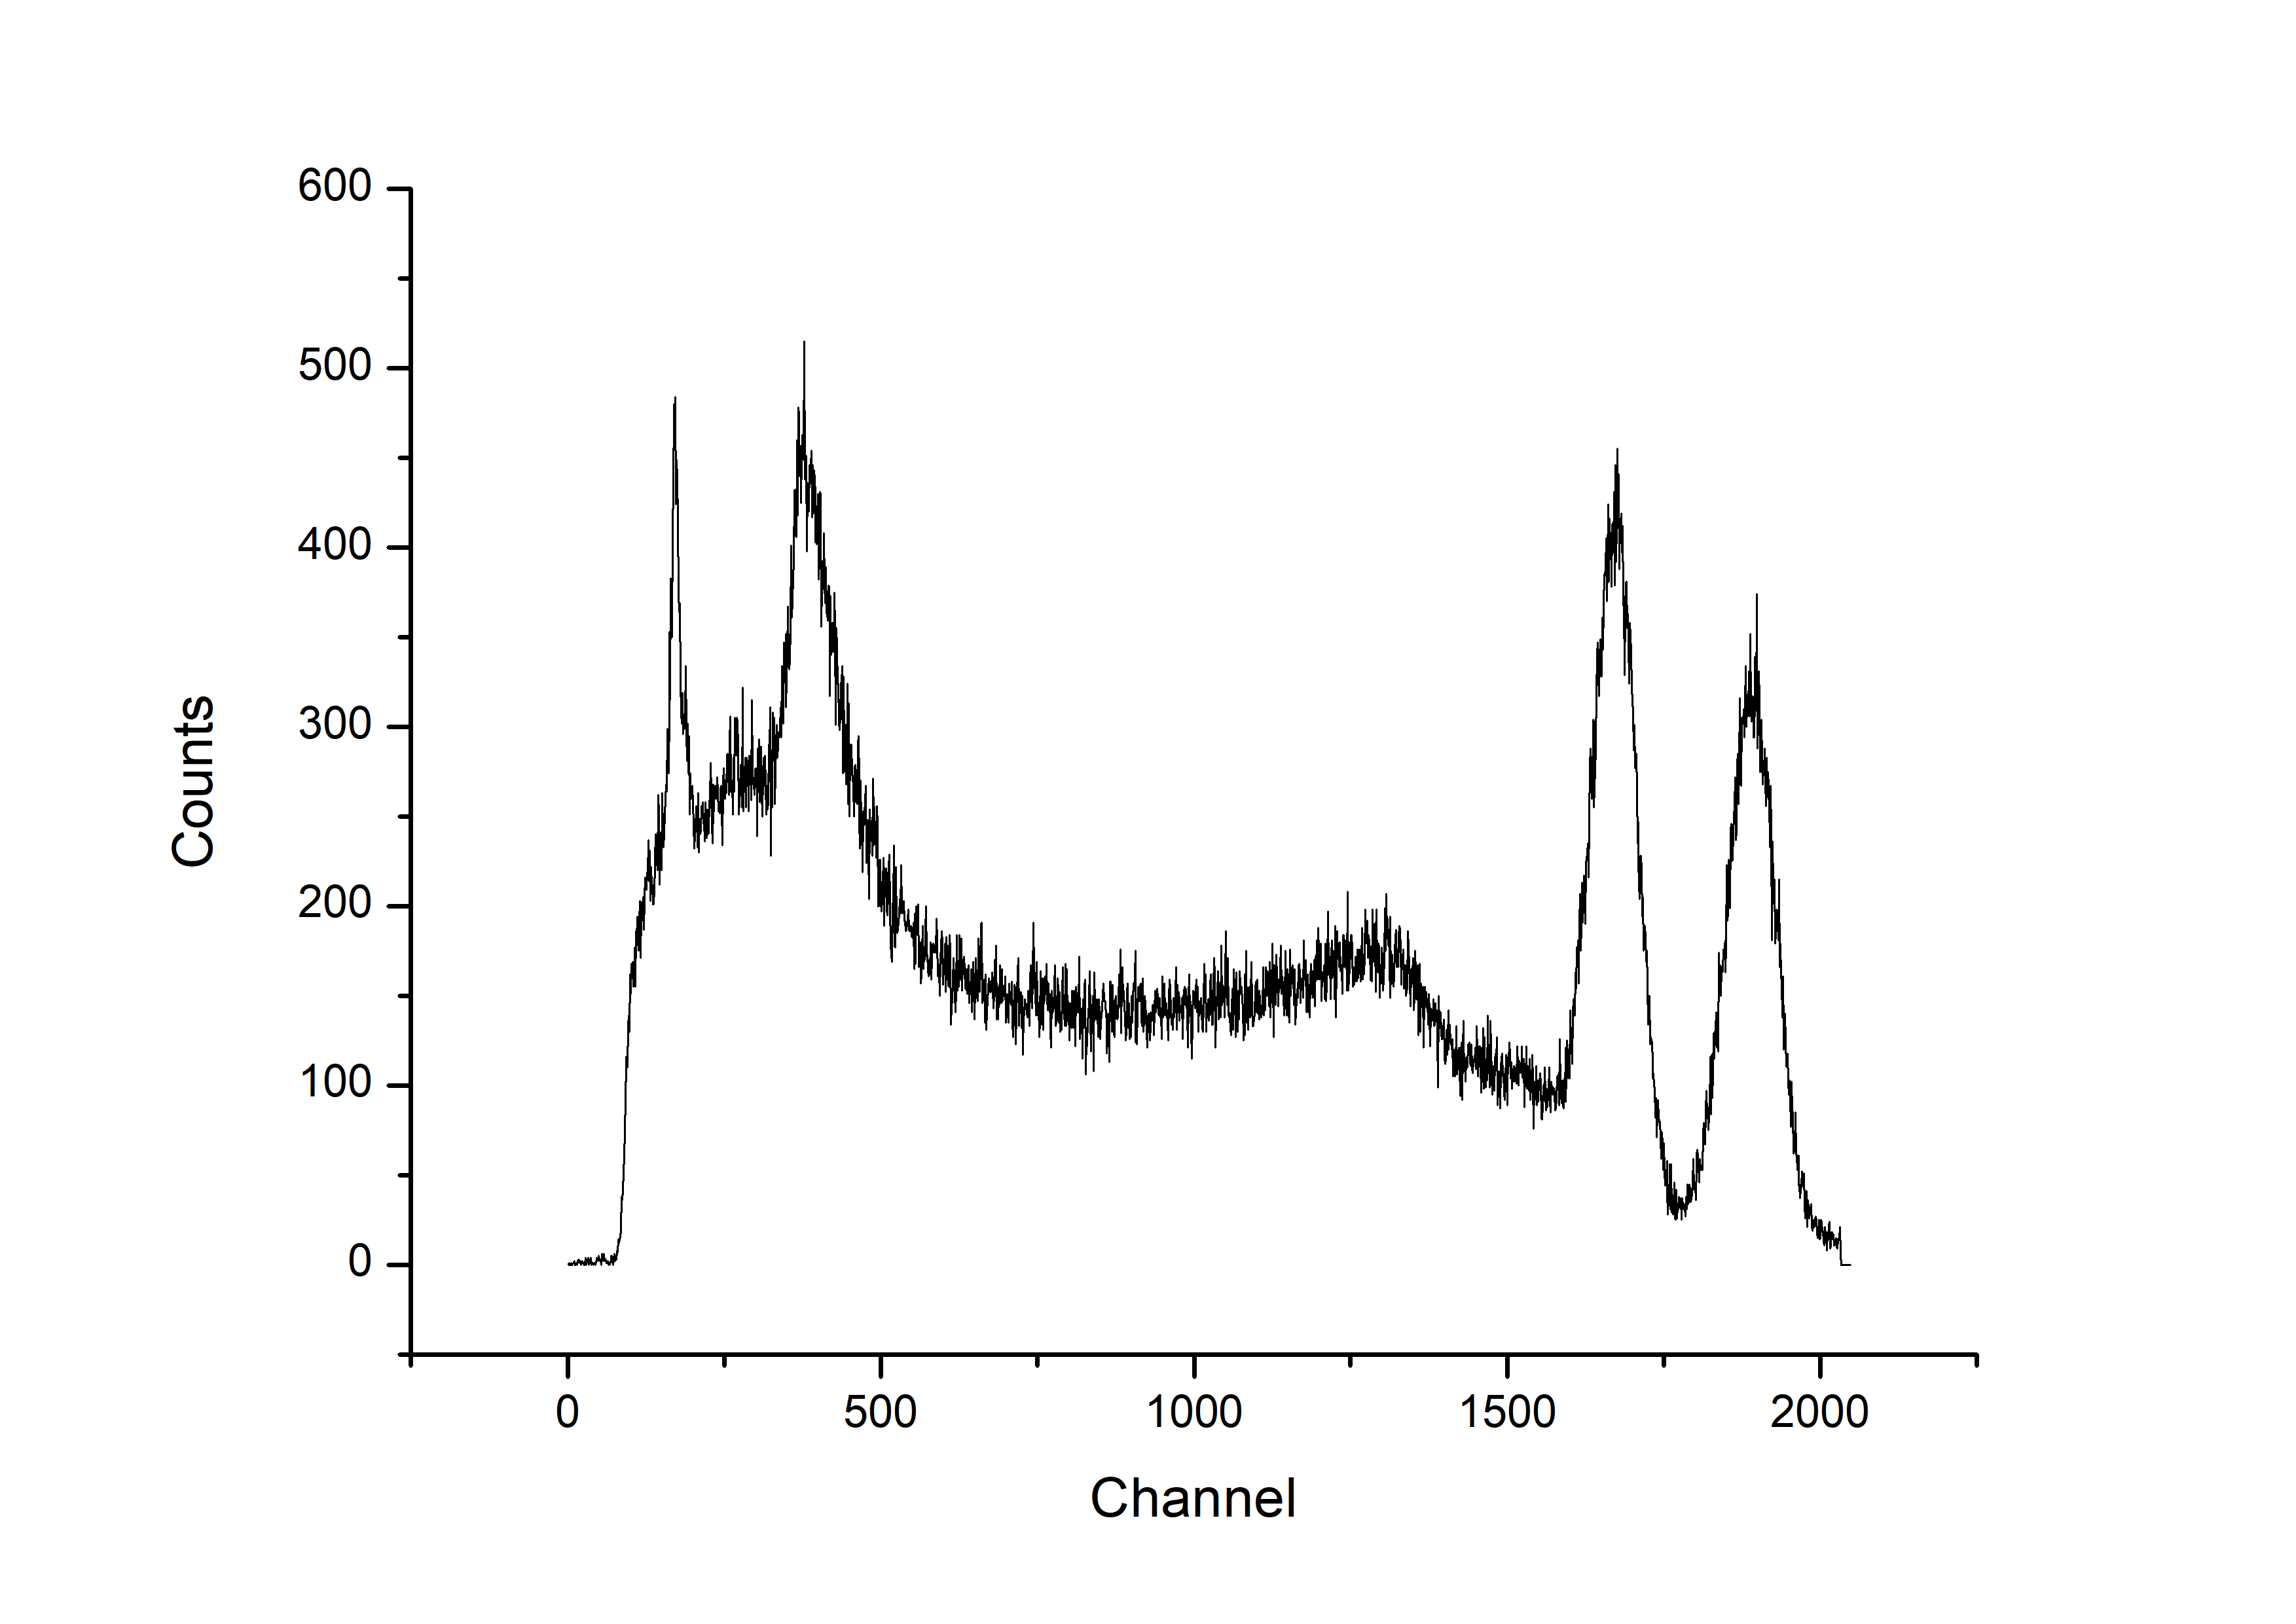
\includegraphics[width=1\linewidth]{image/Co.png}
\caption{Спектр $^{60}$Co}
\end{minipage}
\end{center}
\end{figure}

\begin{figure}[ht]
\begin{center}
\begin{minipage}[ht]{0.48\linewidth}
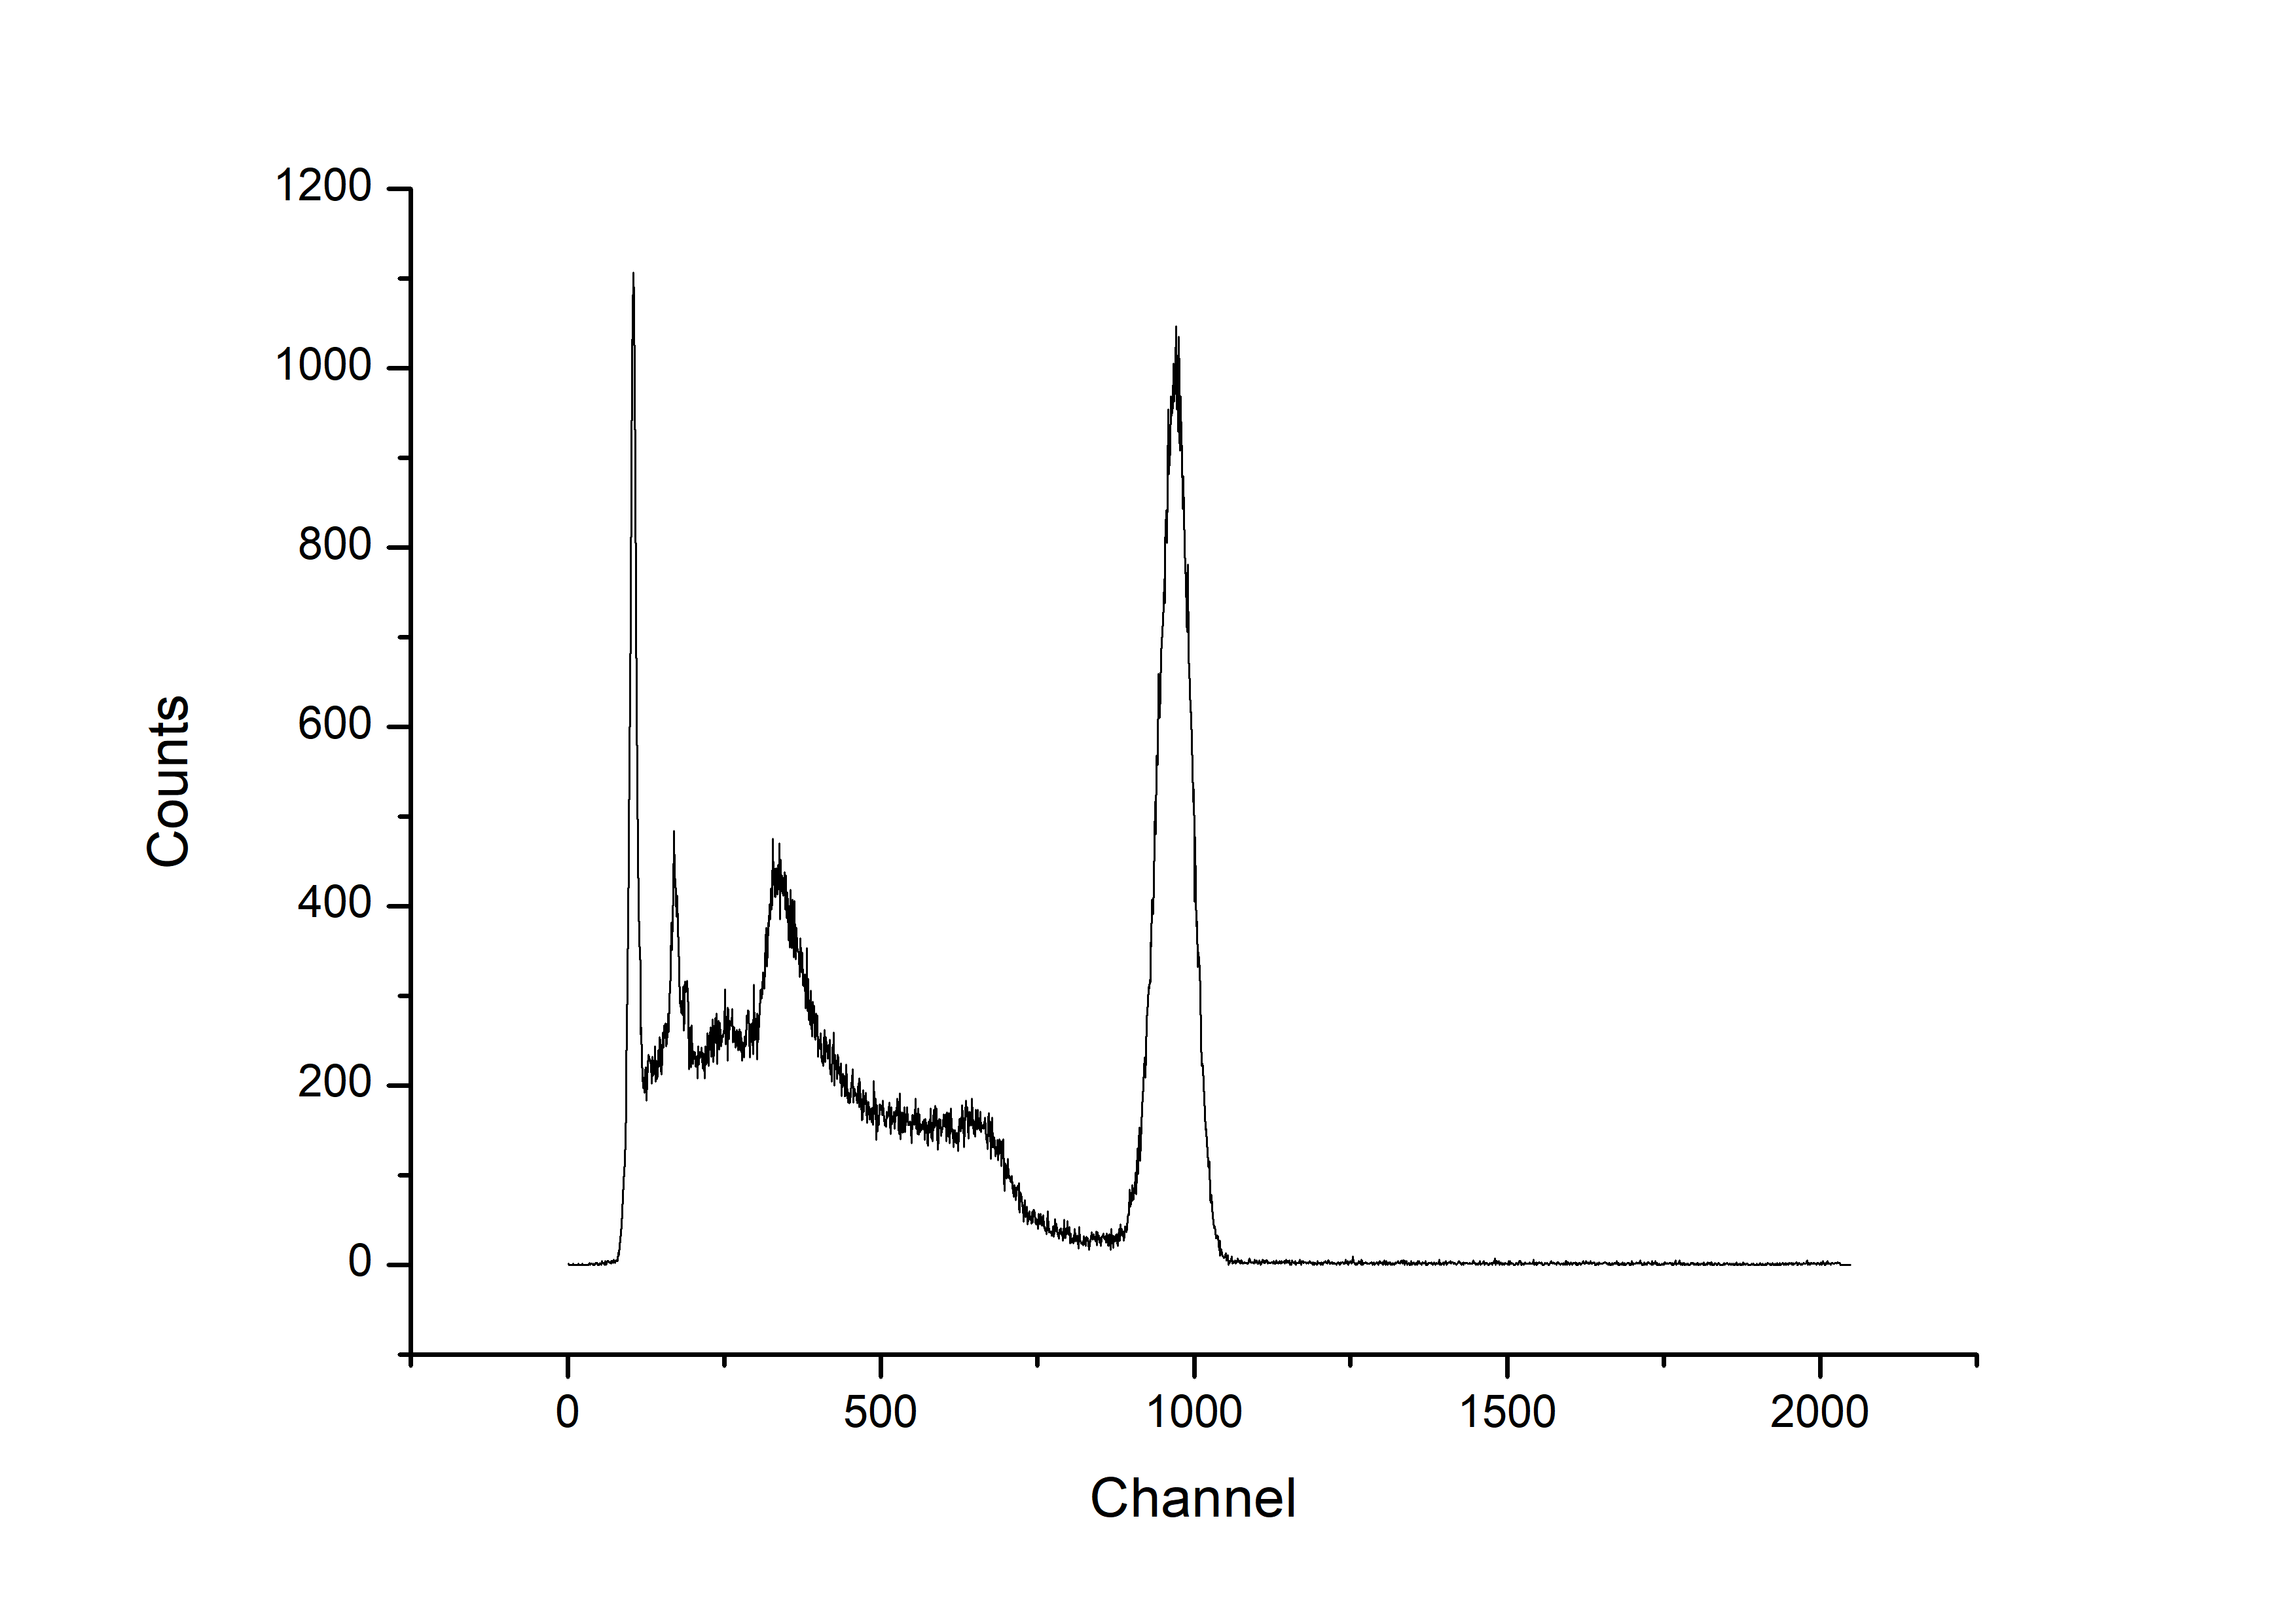
\includegraphics[width=1\linewidth]{image/Cs.png}
\caption{Спектр $^{137}$Cs} %% подпись к рисунку\label{ris:experimoriginal} %% метка рисунка для ссылки на него
\end{minipage}
\hfill 
\begin{minipage}[ht]{0.48\linewidth}
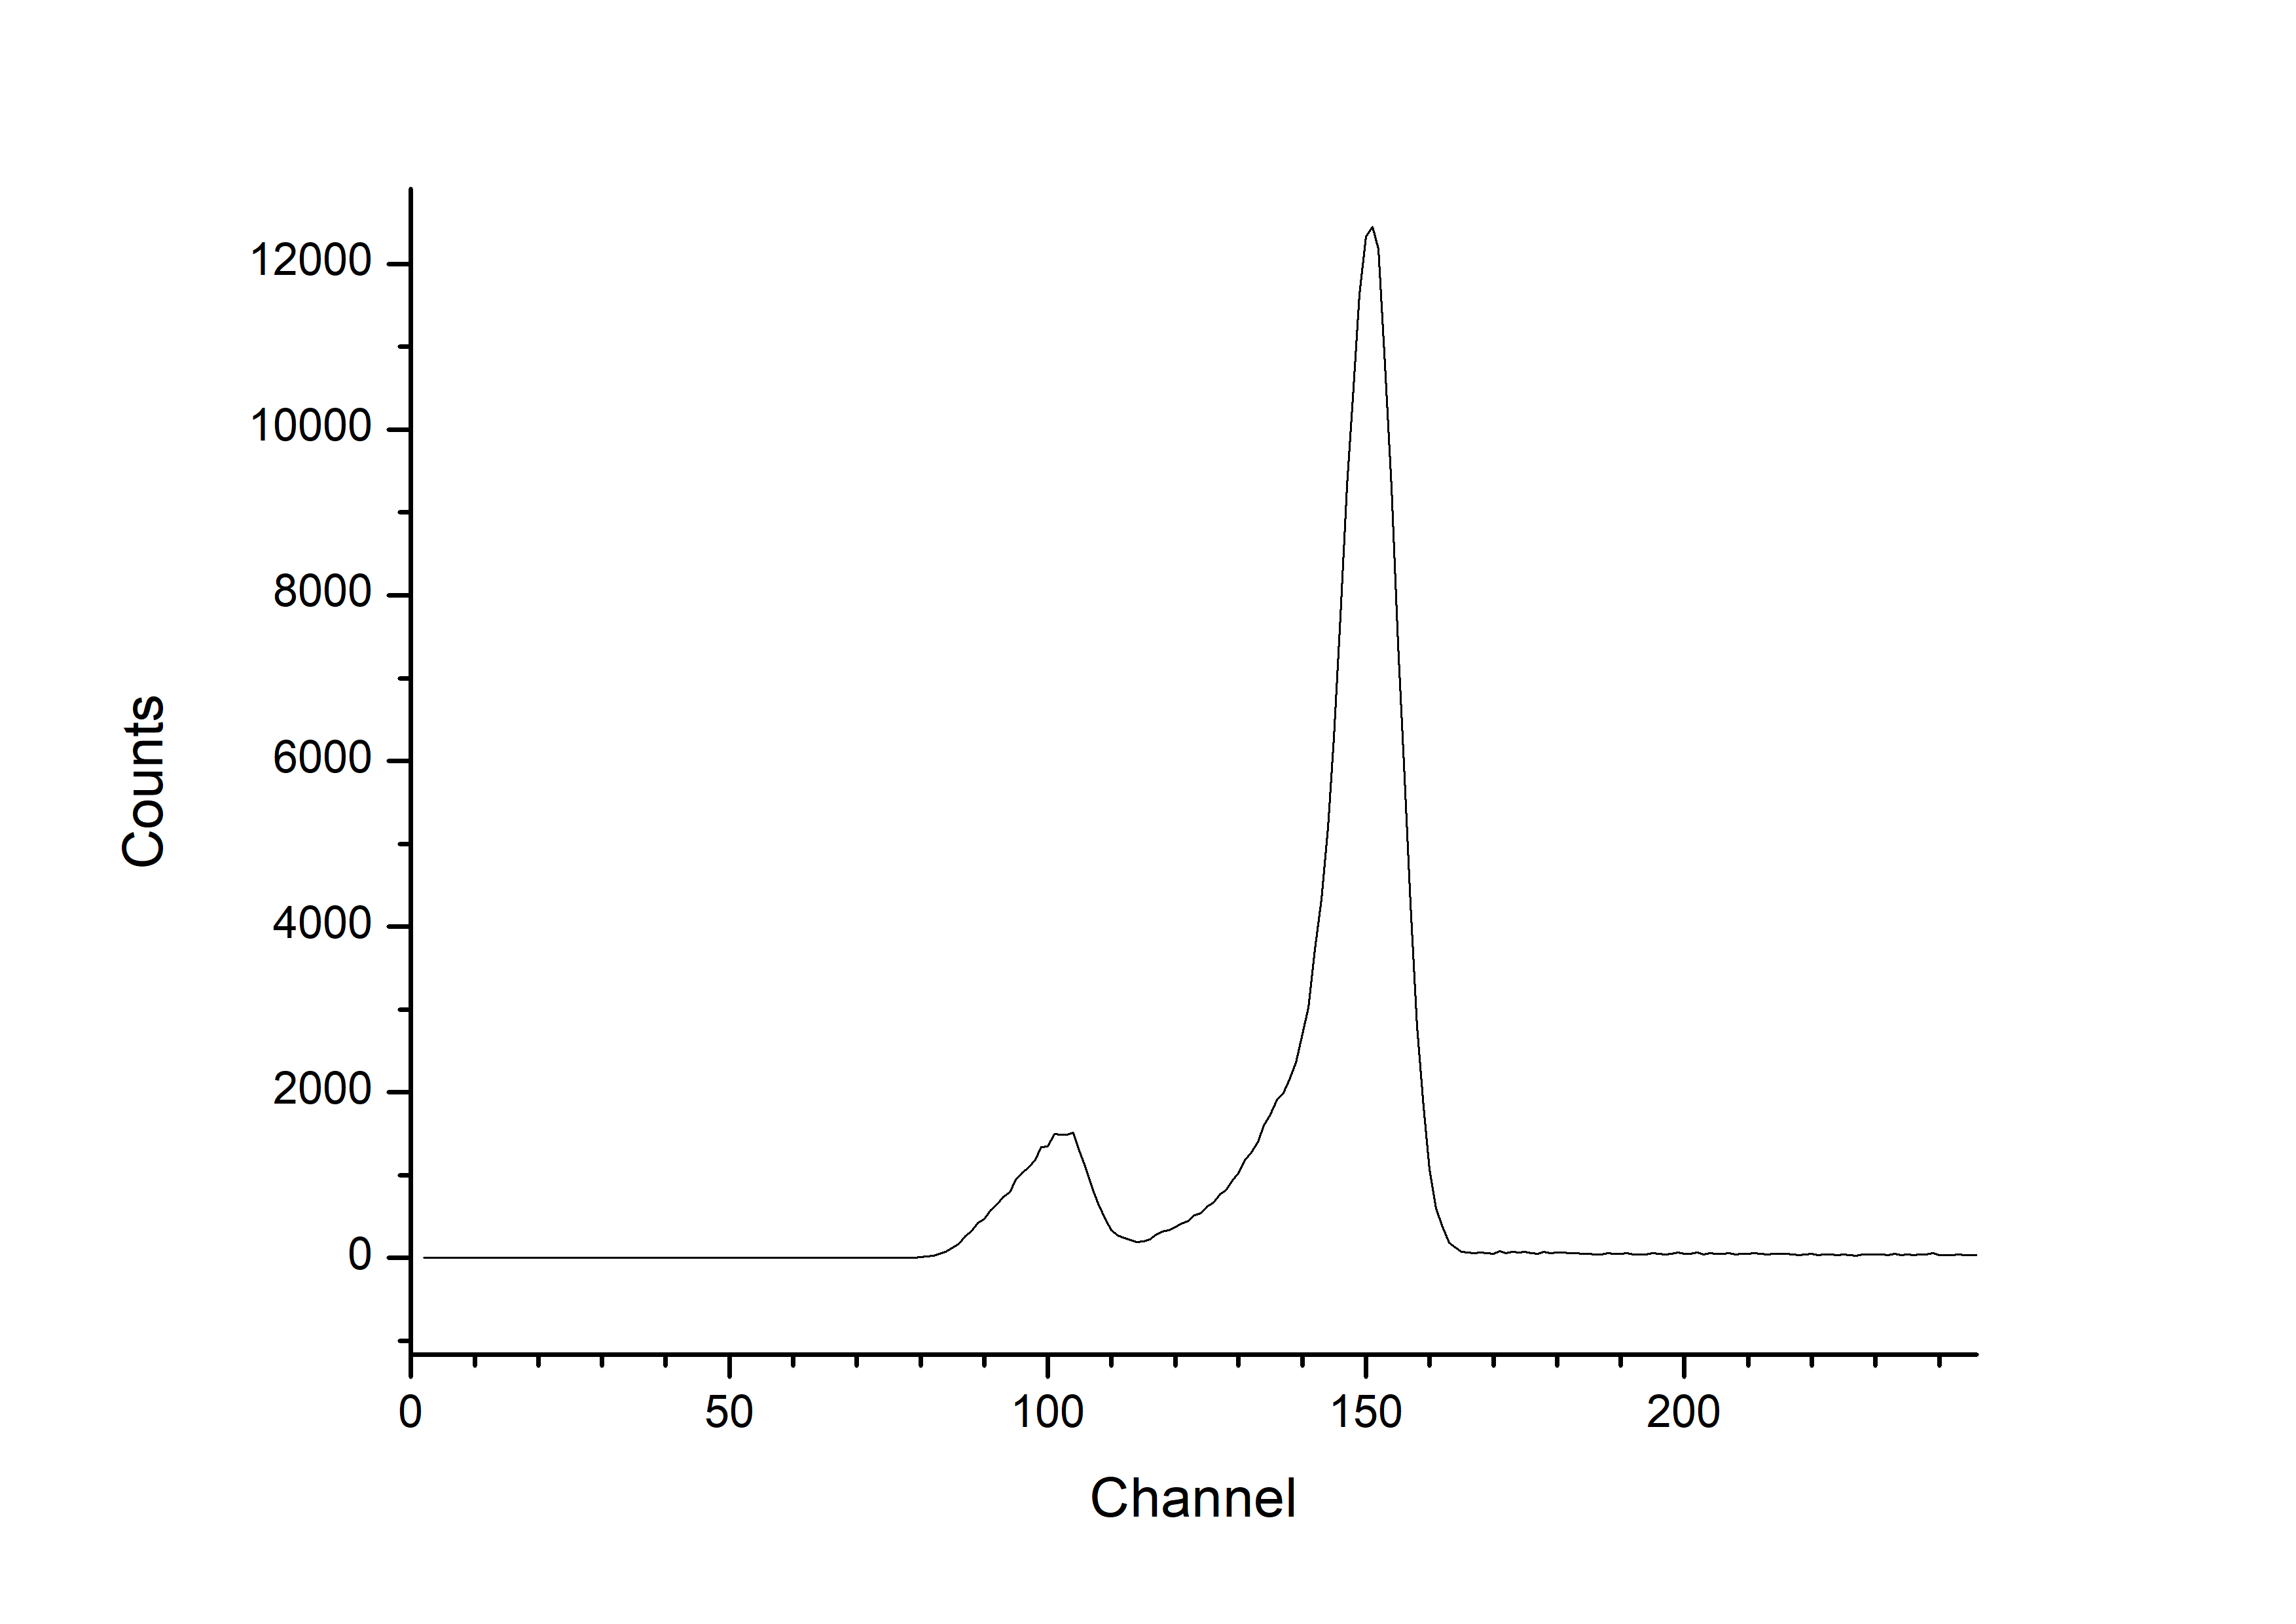
\includegraphics[width=1\linewidth]{image/Am.png}
\caption{Спектр $^{241}$Am}
\end{minipage}
\end{center}
\end{figure}

\begin{figure}[ht]
\begin{center}
\begin{minipage}[h]{0.48\linewidth}
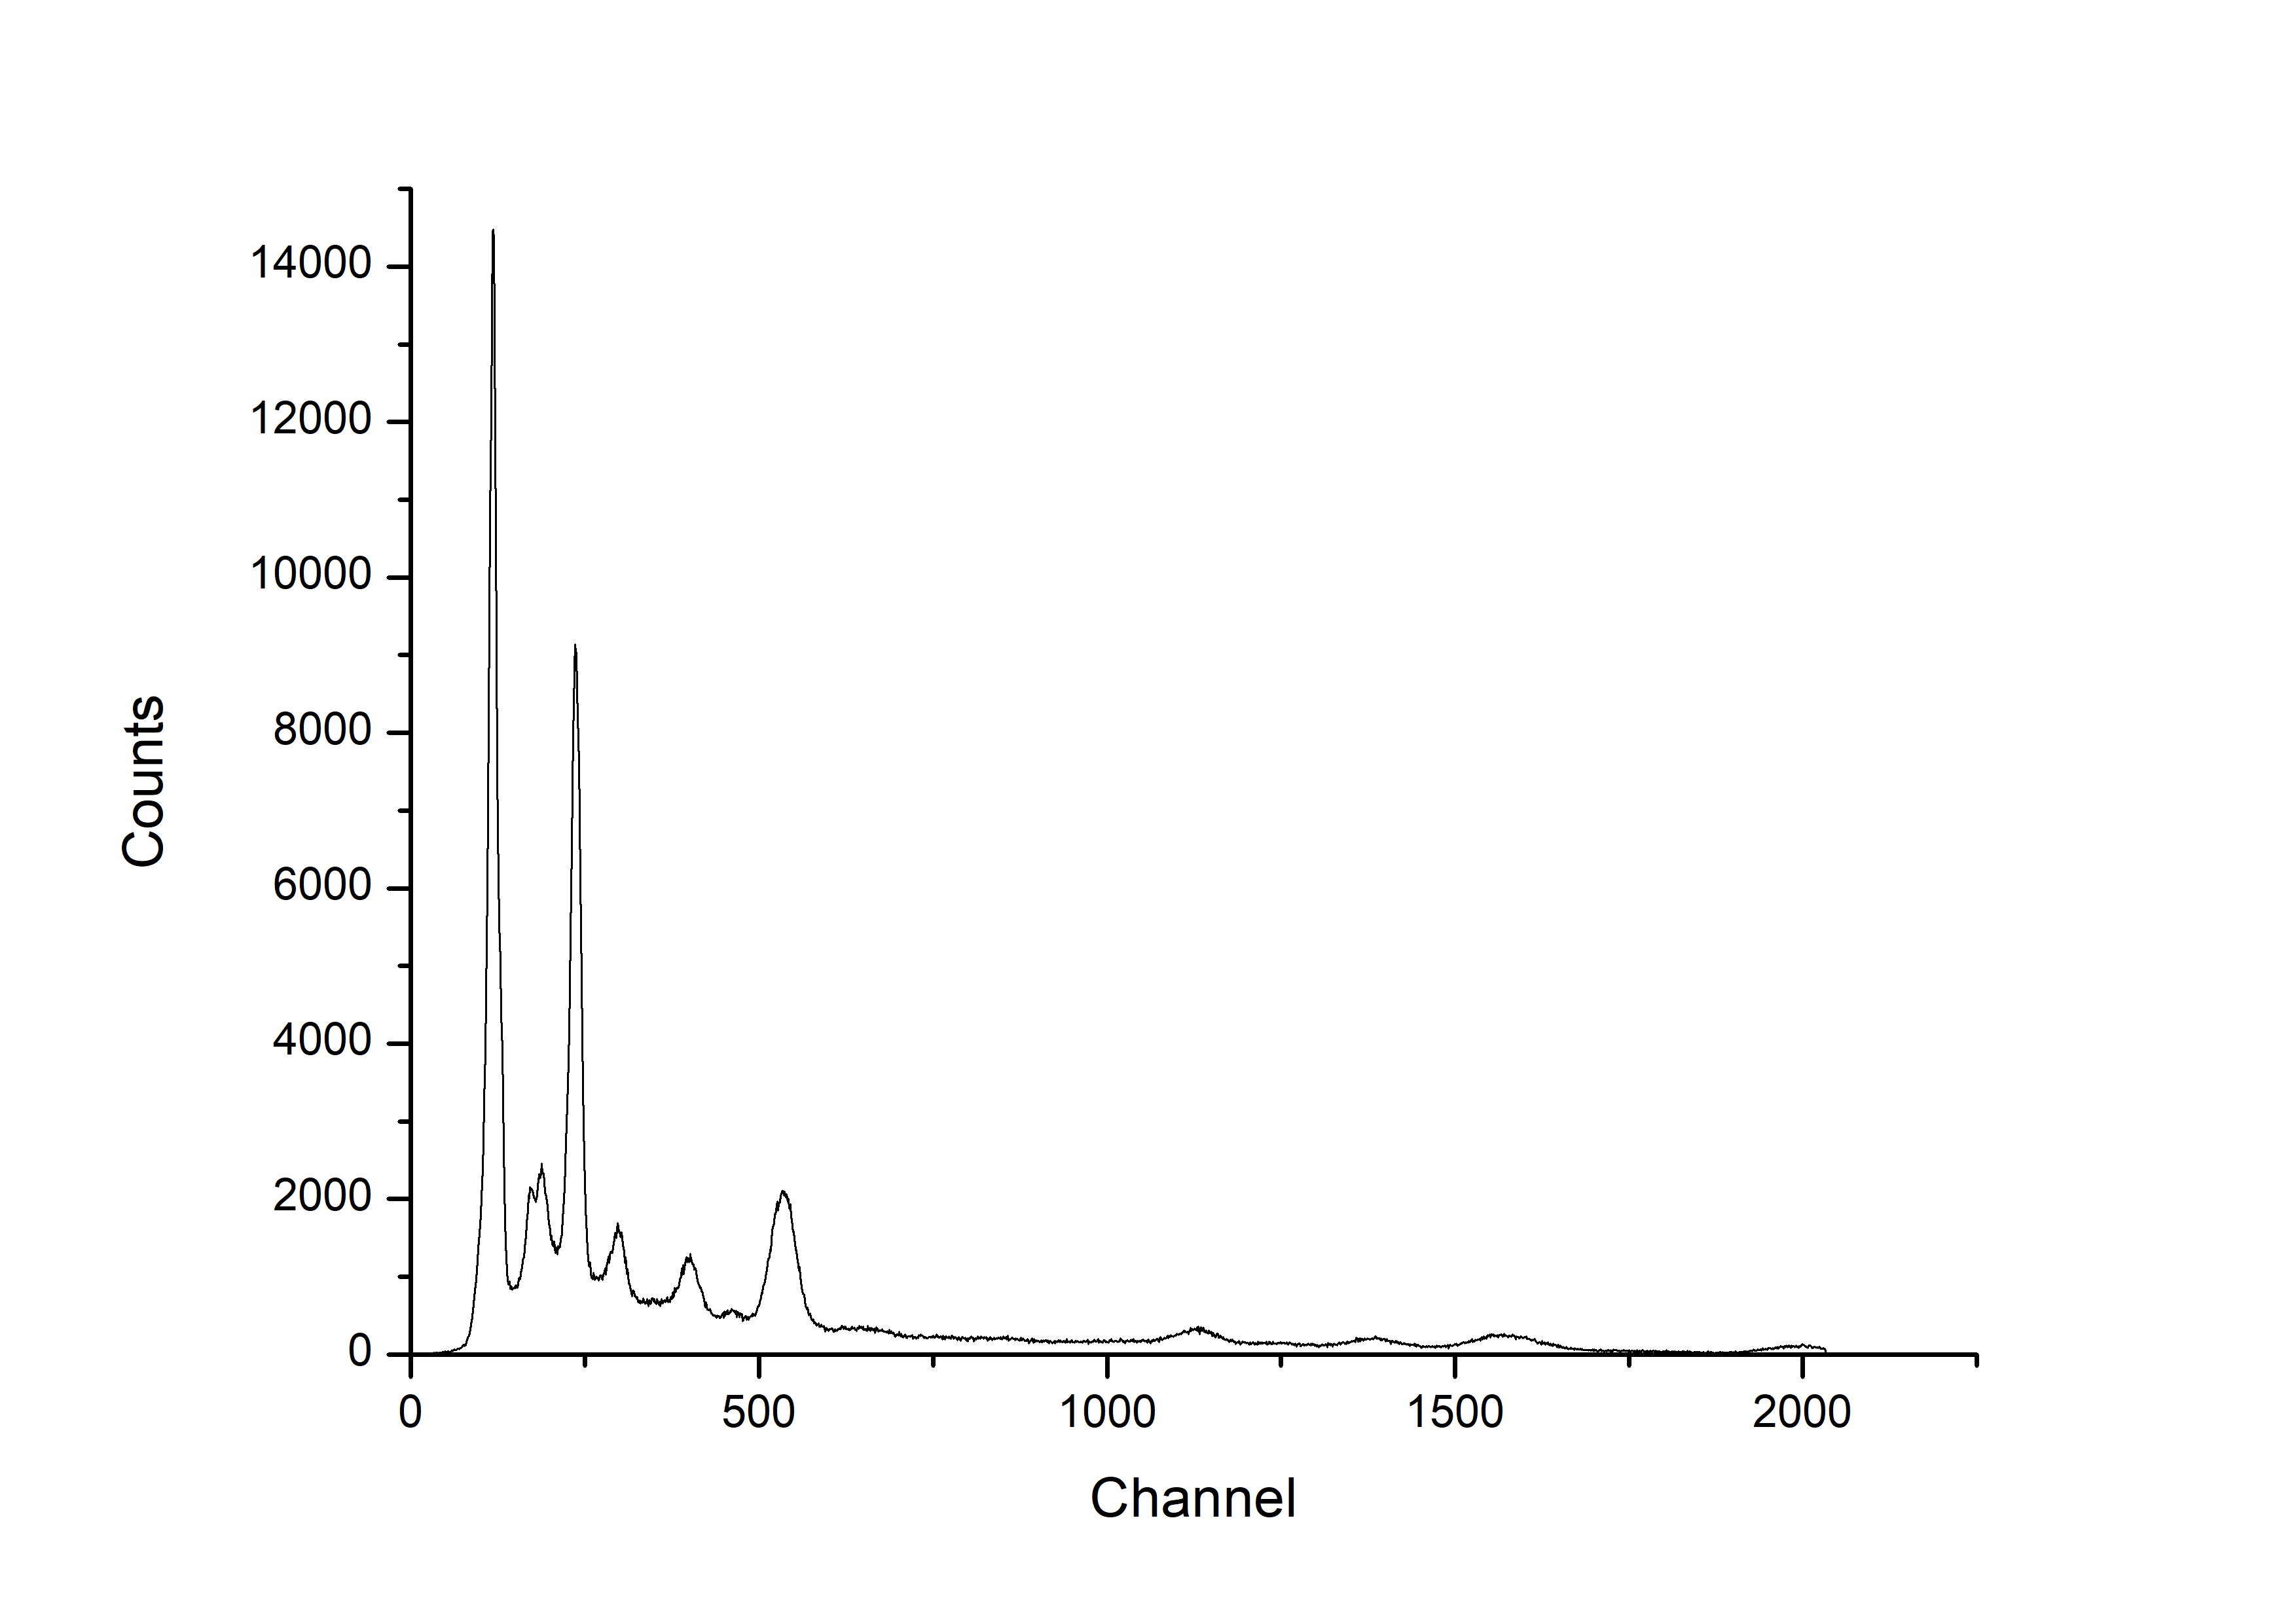
\includegraphics[width=1\linewidth]{image/Eu.png}
\caption{Спектр $^{152}$Eu} %% подпись к рисунку\label{ris:experimoriginal} %% метка рисунка для ссылки на него
\end{minipage}
\hfill 
\begin{minipage}[ht]{0.48\linewidth}
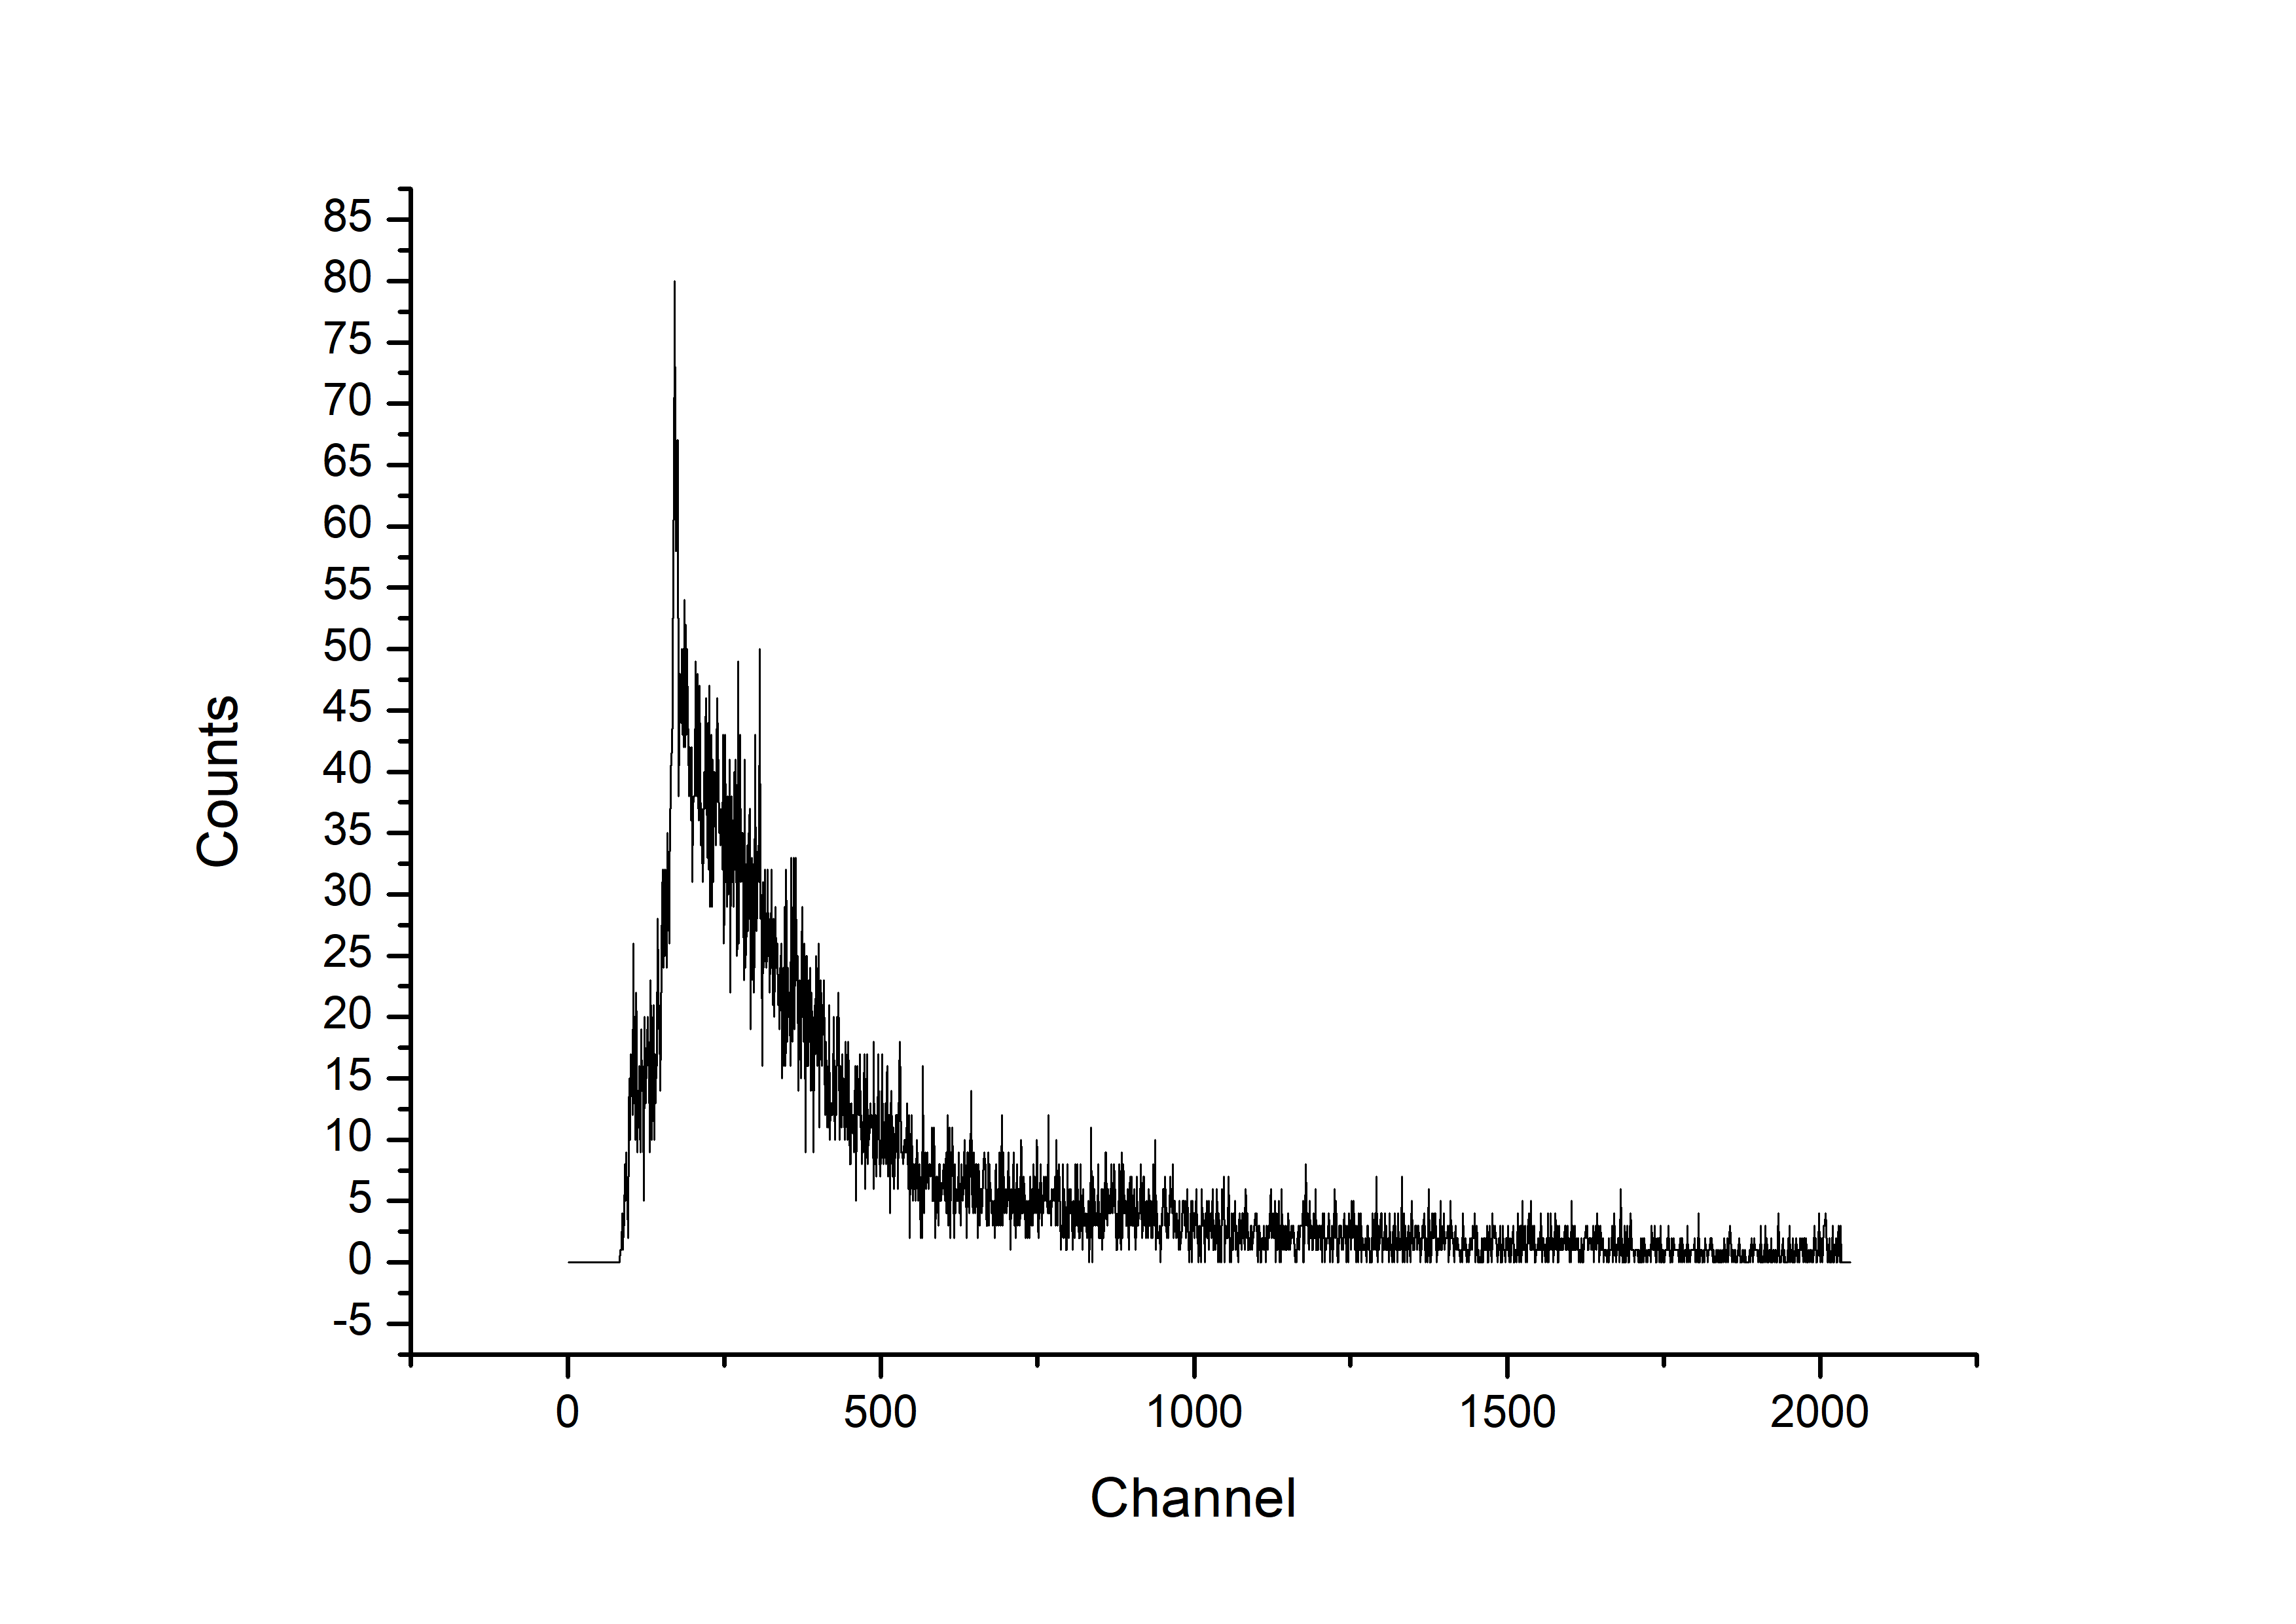
\includegraphics[width=1\linewidth]{image/background.png}
\caption{Спектр шума}
\end{minipage}
\end{center}
\end{figure}

\end{document}
